\chapter{Tail-Anchored Protein Datasets}
\sloppy
% gls refers to a glossary term, cite refers to an entry from the separate bibtex folder. url is a lazy way of forcing monospaced text. textit is italics. sections and subsections are the headers.
\section{Abstract}

\section{Introduction}
This study aims to identify \gls{snare} proteins in eukaryotic proteomes by filtering through large datasets using automatically predicted TrEMBL consensus, and manually annotated SWISS-PROT transmembrane regions.
The pipeline generates a list of singlepass proteins with a transmembrane domain close to the C terminal, that are not splice isoforms.
A previous study predicted 411 tail anchor proteins~\cite{Kalbfleisch2007}.

~\gls{ta} proteins are a topologically distinct class of intracellular proteins defined by their single carboxy-terminal~\gls{tms} with a cytosolic facing amino-terminus.
~\gls{ta} proteins are involved in a range of key cellular functions including protein translocation and apoptosis.
Additionally, within the~\gls{ta} class of proteins are a set of vesicle fusion proteins called~\gls{snare} proteins.
There is biomedical interest in~\gls{snare} drug delivery mechanisms.
~\gls{snare}s can fuse liposomes containing various drug payloads into the membrane.

The pipeline generates a list of singlepass proteins with a transmembrane domain close to the C terminal, that are not splice isoforms.
A previous study by Kalbfleisch \textit{et al.} published in Traffic 2007 (8: 1687-1694) predicted 411 tail anchor proteins~\cite{Kalbfleisch2007}.
The tools developed herein are openly available for re-application to other datasets.
Notably, known~\gls{snare} transmembrane helices are highly hydrophobic even compared to other~\gls{ta} transmembrane helices.
We compare Kyte and Doolittle hydrophobicity profiles of our filtered human protein list against the profiles of previously known~\gls{snare} and~\gls{ta} proteins.
This provided a list of potential~\gls{snare} proteins in addition to potential spontaneously inserting~\gls{ta} proteins similar to cytochrome b5 which have the least hydrophobic transmembrane helices.

Tail-anchored proteins are a topologically distinct class of intracellular proteins defined by their single carboxy-terminal transmembrane domain with a cytosolic-facing amino-terminus.
%Need a figure here of a crystal structure TA.

Tail-anchored proteins are involved in a range of key cellular functions including protein translocation and apoptosis.
Additionally, within the tail-anchored class of proteins are a set of vesicle fusion proteins called \gls{snare} proteins.
There is biomedical interest in \gls{snare} drug delivery mechanisms.

\gls{snare}s can fuse liposomes containing various drug payloads into the membrane.
Notably, known \gls{snare} \gls{tmh}s are highly hydrophobic even compared to other tail anchored \gls{tmh}s~\cite{Kalbfleisch2007}.
This hydrophobicity appears to be a determinate factor in the precise delivery mechanistic route that a~\gls{ta} proteins use for insertion~\cite{Rabu2008, Rabu2009}, for which there is evidence demonstrating that are several mechanisms~\cite{Rabu2009, Johnson2013}.

Whilst most eukaryotic~\gls{ta} proteins are inserted into the~\gls{er}.

\section{Results}

\subsection{Tail-Anchored Protein Datasets Are A Moving Target}
% Venn diagram
\begin{figure}[!ht]
\centering
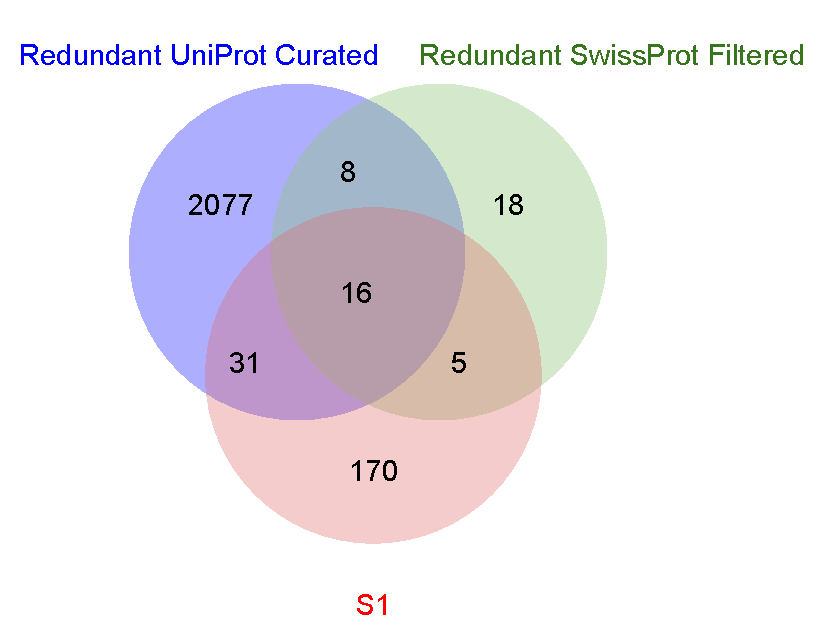
\includegraphics[width=0.5\textwidth]{TA_chapter/database-overlap}
		\captionof{figure}[A venn diagram showing tail anchored protein UniProt ids present in each of the datasets as well as those present in multiple datasets.]{\textbf{A venn diagram showing tail anchored protein UniProt ids present in each of the datasets as well as those present in multiple datasets.}
The number of ids present in redundant versions of
i) the supplementary materials table of a previous study predicting the complete set of human tail anchored proteins denote by S1~\cite{Kalbfleisch2007},
ii) the Swissprot dataset filtered according to typical~\gls{ta} features limited to the human proteome~\cite{TheUniProtConsortium2014}, and
iii) The UniProt curated list of~\gls{ta} proteins~\cite{TheUniProtConsortium2014}.
Note that to avoid losing IDs to redundancy reduction this diagram was generated without the use of CD-HIT~\cite{Huang2010, Wu2011}, which is applied in later statistical analysis.}

\label{fig:tadatasetoverlap}
\end{figure}

Datasets are a moving target as they are constantly updated with more accurate and reliable tools.
Figure~\ref{fig:tadatasetoverlap} shows that already a study from 2007~\cite{Kalbfleisch2007} has 175 record ids of 222 records (78.8\%) that do not share overlap the up-to-date manually curated UniProt dataset~\cite{TheUniProtConsortium2014}.
Of the 166 unique records, 92 records do have location annotation in UniProt that the scripts herein use for topological determination, leaving 74 records without location annotation.
This leaves 92 of 222 (41.4\%) records that originally fitted criteria that no longer fit those same criteria. If we exclude those lacking suitable annotation i.e ids from S1 that are found in either SwissProt with the filters (9), the curated UniProt list (14), or both (33), compared to the 92 that have annotation contradicting the original prodictions, 37.8\% of the ids overlap.

Equivalent criteria were applied to the entire SwissProt database and then restricted to the human proteome dataset.
43 of these 77 records are in the curated UniProt~\gls{ta} dataset leaving 34 records that meet the criteria out of the manually curated set (44.2\%of the filtered Swissprot dataset).
42 of the 77 (54.5\%) records from SwissProt filtered human dataset can be found in the original S1 list.

Perhaps unsurprisingly, as a trend this shows that up to date datasets drastically improve the reliability of this automated predicted method and that there is a large degree of what we now believe to be mistakes that occured in older prediction tools.
These automated criteria still do not fully align with the manually curated list, which is bound to change too.

Note that these numbers are not absolutely certain.
The greatest source of uncertainty here is that the original S1 list includes 411 records, however only 222 of these were successfully mapped to the UniProt dataset, which prevents us from directly comparing the entire original S1 dataset.

\subsection{Species Variation}
% Average lines for figure, table for stats

\subsection{Organelle Membrane Variation}
% Average lines for figure, table for stats

\subsection{SNAREs are consistently more hydrophobic across the entire \gls{tmh}}
% Average lines for figure, table for stats

~\gls{snare} proteins were noted to have more of the most hydrophobic amino acids than the general population of tail anchors~\cite{Kalbfleisch2007}.
We exploit the difference by mapping the hydrophobicity of the transmembrane domains from a novel list of potential~\gls{ta} proteins generated in this study onto the experimentally validated~\gls{ta} hydrophobicity plot compiled by Kalbfleisch et al. published in Traffic 2007 (8: 1687-1694) (Figure 3).
This method has revealed potential~\gls{ta}~\gls{snare}s with~\gls{snare} motif domains that may not appear in conventional screening.

\subsection{Spontaneous insertion may be achieved by polar patches in the \gls{tmh}}
%Spont TA lines against background dataset.

In addition, predicted insertion machinery dependent TAs with TMHs that are more polar on average than spontaneously inserting~\gls{ta} protein cytochrome b5 have been highlighted.

%move on to case studies involving spontaneous insertion?
Signal anchored proteins, proteins that contain a single hydrophobic segment that serves as both a mitochondrial targeting signal and a membrane anchor, as well as tail-anchored proteins have been shown to be able to spontaneously insert into the membrane independently from the translocon~\cite{Elisa2012, Lan2000, Colombo2009}.

It is postulated that there are electrostatic factors in the flanking regions that contribute to this spontaneous membrane insertion.
Our experimental collaborators in Stephen High’s group are interested in a small group of tail-anchored proteins that have very polar trans-membrane domains and are capable of liposome membrane insertion without insertion machinery, also known as spontaneous insertion.
They have found that chimeric synaptobrevin, one of the first identified \gls{snare} proteins, is capable of spontaneous insertion if the tail anchor domain is replaced by the \gls{tm} domains belonging to a protein of known spontaneously inserting domains.
Their studies have moved the focus of spontaneous insertion away from the loop regions and onto the physicochemical factors of the \gls{tmh} itself.
The idea that \gls{snare} proteins are modular and capable of spontaneous insertion has significant implications for both biomedical application in liposome-based drug delivery and can aid future research for testing complex biological molecular networks~\cite{Allen2013, Nordlund2014}.

\section{Methods}

\subsection{Building a List of Tail-Anchors}
Steps carried out by Kalbfleisch \textit{et al.} published in Traffic 2007 (8: 1687\-1694)~\cite{Kalbfleisch2007}, were recreated using up to date tools. Whilst their study focussed on the human proteome, here we take into account the entire TrEMBL and Swiss-Prot database and then stratify the datasets by the organism at the end of the pipeline.

\subsubsection{Swiss-Prot Tail Anchored Dataset According to Filters}
There were 557012 protein records downloaded from Swiss-Prot via UniProt~\cite{TheUniProtConsortium2014} (Downloaded 24--04--2018).
106149~\gls{tmh}s (\url{TRANSMEM} annotation) were found between 76953 records (\url{annotation:(type:transmem) AND reviewed:no}).
This keyword is contained in a record according to either experimental evidence~\cite{TheUniProtConsortium2014} or a robust meta-analysis of~\gls{tmh} prediction using TMHMM~\cite{Krogh2001}, Memsat~\cite{Jones2007}, Phobius~\cite{Kall2004,Kall2007} and the hydrophobic moment plot method of Eisenberg and co-workers~\cite{Eisenberg1984}.
11141 of those records had only a single~\gls{tmh}.
11110 of those~gls{tmh}s were within the length thresholds of 16 to 30 residues (None of those had the annotation for splice isoforms according to \url{NON_TER} annotation).
5548 of those had had no~\gls{sp} annotation (\url{SIGNAL}).
4332 of those had annotation (based on \url{TOPO_DOM} annotation) that the N terminal was cytoplasmic.
615 of those had the~\gls{tmh} within 25 residues of the C terminal, the same threshold used by Kalbfleisch and their coworkers~\cite{Kalbfleisch2007}.
Running CD-Hit 4.5.3 on the WebMGA webserver~\cite{Huang2010, Wu2011} at 90\% identical sequence at 90\% coverage thresholds resulted in 443 representative proteins.
This threshold was chosen as a compromise between avoiding over-representation of a certain protein and maintaining a viable sample size.
%I do not like the next line.
Even though this allows potentially identical~\gls{tmh}s to be included in analyses, that alone has value providing it is not the same protein.
From this representative list, 46 were Archaeal, 66 were bacterial, and 320 were Eukaryotic and 11 came from dsDNA viruses.
49 belonged to the \textit{A. thaliana} proteome, 48 to Mouse, 46 to the human proteome, 24 to Rat.

\subsubsection{TrEMBL Tail Anchored Dataset According to Filters}
111425234 records were storeed in the TrEMBL database at time of download (Downloaded 25--04--2018).
22107826 of those contained \url{TRANSMEM} annotation (\url{annotation:(type:transmem) AND reviewed:no}).
18053 of these were single-pass proteins.
All of these were within the length restrictions.
17973 of those did not contain a signal sequence when looking for \url{SIGNAL} annotation.
5157 of those contained a cytoplasmically located N terminal according to \url{TOPO_DOM} annotation.
155 records had a~\gls{tmh} within 15 residues of the C terminal residue.

\subsubsection{UniProt Curated List}
A query for \url{locations:(location:"Single-pass type IV membrane protein [SL-9908]")} was used in UniProt which returned 2460 UniProtKB IDs; 463 Swiss-Prot results and 1997 TrEMBL results.
Running these records through CD-HIT at 90\% redundancy yielded 309 Swiss-Prot records and 808 TrEMBL records~\cite{Huang2010, Wu2011}.
Of those, 987 proteins from 973 records (308 from Swiss-Prot, and 665 from TrEMBL) had the \url{TRANSMEM} annotation indicating a bone fide~\gls{tmh}.
No further filters were applied to this list.
60 of the records belonged to \textit{A. thaliana}, 38 to Humans, 37 to mouse, 31 to \textit{S. cereveisiae}, and 20 to Rat.

\subsubsection{Remapping Previous Dataset}
189 of the 411 proteins from the previous study were successfully mapped to 222 UniProtKB IDs using the UniProt mapping tools with the RefSeq Protein to UniProtKB option~\cite{TheUniProtConsortium2014}.

\subsection{Calculating Hydrophobicity}
Windowed hydrophobicity was calculated using a window length of 5 residues, and half windows were permitted.
Average hydrophobicity takes the total of the raw amino acid hydrophobicity values and divides them by the number of amino acids in the slice.
Values reported in the results are based on the Kyte \& Doolittle scale~\cite{Kyte1982} which is based on the water\---vapour transfer free energy and the interior-exterior distribution of individual amino acids.
Hydrophobicity values were also validated by the White and Wimley scale~\cite{White1999}, the Hessa scale~\cite{Hessa2005}, and the Eisenberg scale~\cite{Eisenberg1984}.
